\documentclass[11pt]{standalone}
\usepackage{pgf, tikz}
\usetikzlibrary{arrows, automata}

\begin{document}
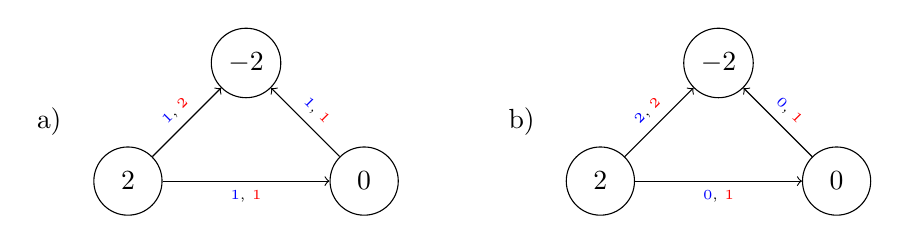
\begin{tikzpicture} [align=center]
\path (-1, 0.75) node (a) {a)}
      (0, 0) node[circle, draw, text width=0.5cm] (v0) {$2$}
 	  (3, 0) node[circle, draw, text width=0.5cm] (v1) {$0$}
	  (1.5, 1.5) node[circle, draw, text width=0.5cm] (v2) {$-2$};
	  
\draw[->] (v0) to node [sloped, anchor=center, below] {\tiny \textcolor{blue}{1}, \textcolor{red}{1}} (v1);
\draw[->] (v0) to node [sloped, anchor=center, above] {\tiny \textcolor{blue}{1}, \textcolor{red}{2}} (v2);
\draw[->] (v1) to node [sloped, anchor=center, above] {\tiny \textcolor{blue}{1}, \textcolor{red}{1}} (v2);

\path (5, 0.75) node(b) {b)}
      (6, 0) node[circle, draw, text width=0.5cm] (v3) {$2$}
	  (9, 0) node[circle, draw, text width=0.5cm] (v4) {$0$}
	  (7.5, 1.5) node[circle, draw, text width=0.5cm] (v5) {$-2$};
      
\draw[->] (v3) to node [sloped, anchor=center, below] {\tiny \textcolor{blue}{0}, \textcolor{red}{1}} (v4);
\draw[->] (v3) to node [sloped, anchor=center, above] {\tiny \textcolor{blue}{2}, \textcolor{red}{2}} (v5);
\draw[->] (v4) to node [sloped, anchor=center, above] {\tiny \textcolor{blue}{0}, \textcolor{red}{1}} (v5);
\end{tikzpicture}
\end{document}